\chapter{State of the science of methane hydrates}
Methane hydrates are clathrate compounds, which means they consist of host molecules forming a lattice that traps guest molecules. Special to clathrate hydrates, which are clathrates there water form the lattice, is that the structure is stabilized by the guests, and would collapse into regular ice or liquid water without guests present. Metane hydrates are among the more prevalent clathrate hydrates, and are formed by water molecules providing cages that host methane molecules. The most common cage structures are comprised of pentagonal and hexagonal faces forming regular cage stuctures. These structures can be described as replications of relatively simple unit cells. This work focus on methane hydrates, but since other clathrate hydrates have also been researched - and are relevant - they may be briefly discussed.


\section{Molecular structure}
Different hydrate structures form based on the size of the guest molecules. These structures are characterized by what cages they can be divided into. Cages are described with compunds of the notation $x^y$ where $x$ is the number of faces of a cetain type, and $y$ describes the type of face by the number of corners on that face of that type. The most common structures for clathrates with one type of guest molecule are the so called structure I (sI) and structure II (sII). These structures, along with the cages that form them, are illustrated in figure \ref{fig:methane_hydrate_structure}. The sI structure contains $5^{12}$ and $5^{12}6^2$ cages in ratio $1:3$, the sII structure contains $5^{12}$ and $5^{12}6^4$ cages in ratio $2:1$.  

Small guest molecules, such as methane and ethane, usually form sI hydrates if the conditions for hydrate formation are met \cite{Hester2009}. However, that is only certain if the hydrate is either purely methane or purely ethane. For mictures of methane and ethane forming gas hydrates, either sI or sII can be formed, depending on the relative amounts of methane and ethane \cite{Subramanian20001981}. 

Not all cages need to be occupied by a guest molecule, so a pure methane hydrate sample can, in addition to its cage structure, be characterized by its cage occupancy. It is common to use the hydrate number to describe cage occupancy, which for methane hydrate looks like:
\begin{equation}
	\mathrm{CH_4} \cdot n_w \mathrm{H_2O}
\end{equation}
Where $n_w$ is the hydrate number. For a fully occupied sI hydrate, the hydrate number would be $n_w = 5.75$. (observed hydrate number \citet{Circone2005})

\begin{figure}
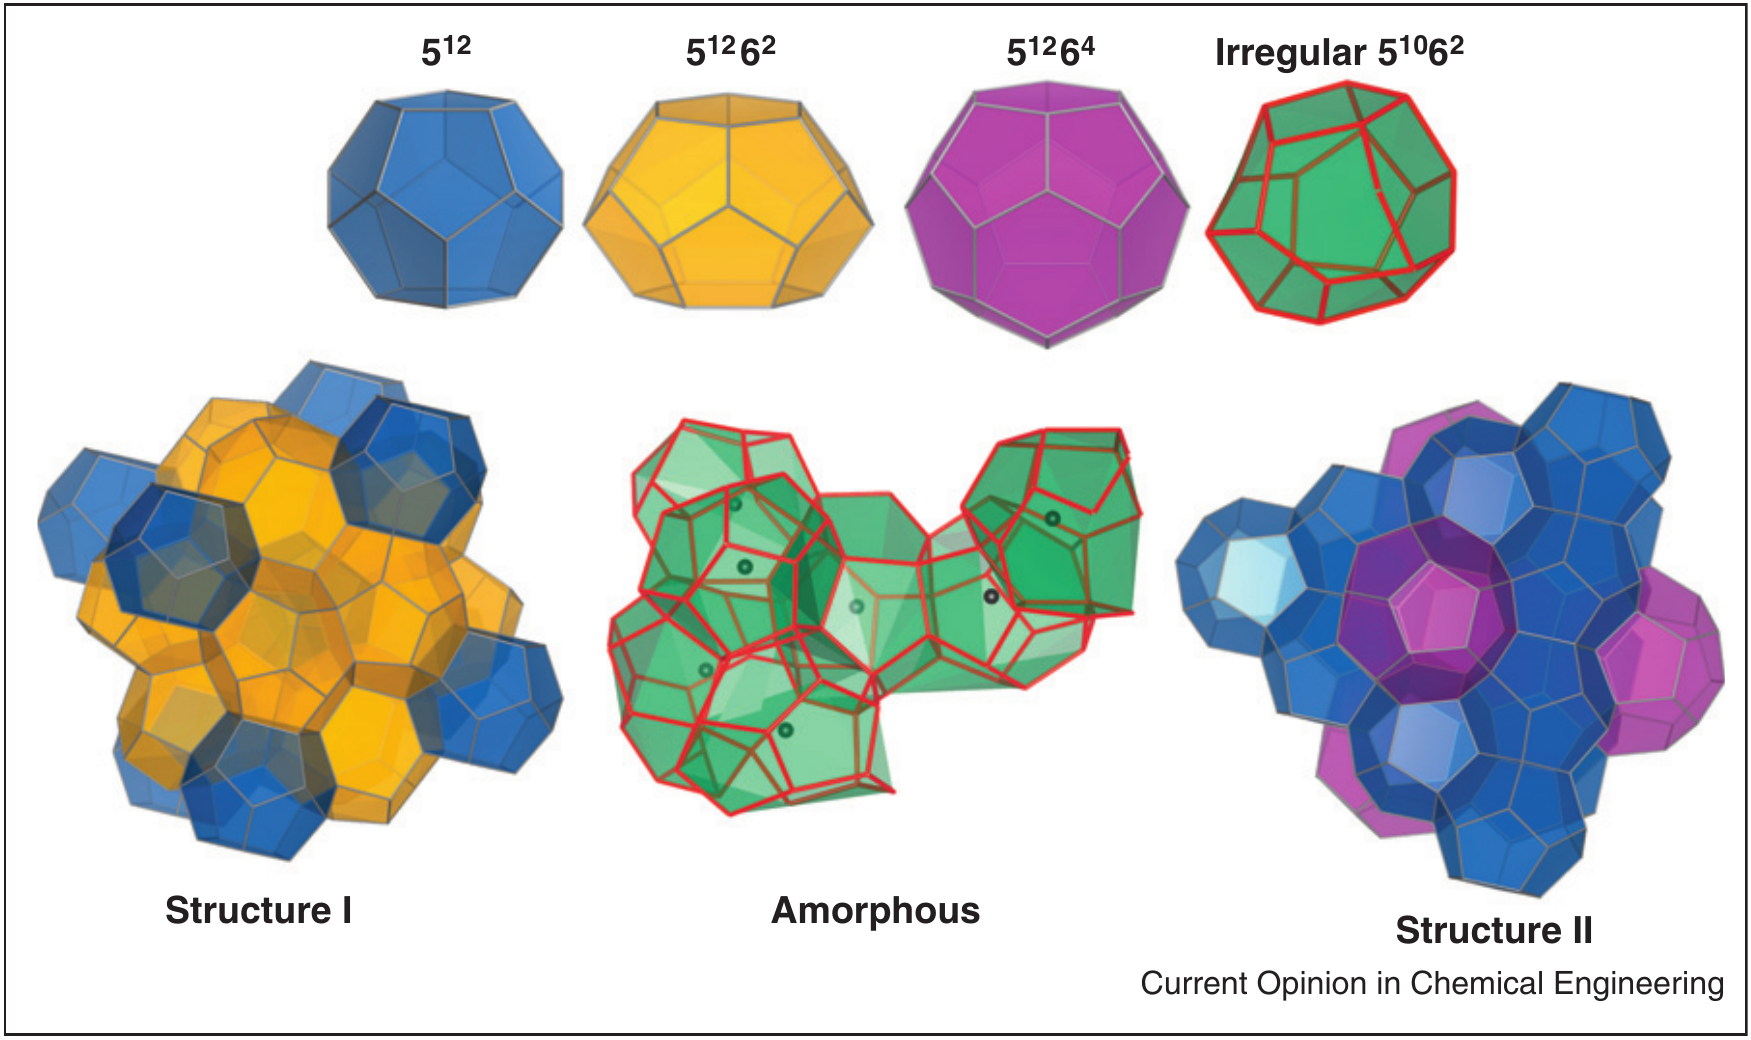
\includegraphics[width=15cm]{../pictures/hydrate_structures.png}
\caption{Cage structures of single guest methane hydrates occuring in nature. Both structure 1 (sI) and structure 2 (sII) contain the $5^{12}$ almost spherical cage. Reprinted from \citet{Barnes2013} with permission from Elsevier.}
\label{fig:methane_hydrate_structure}
\end{figure}


\section{Mechanical properties from experiments}
Since methane hydrates come in many forms, it is hard to say someting general about elastic properties, strength and toughness. In a review paper from 2012, \citet{Ning2012} state:
\begin{quotation}
Few mechanical properties are reported , and their measurements are difficult, partly because it is almost impossible to obtain pure hydrate samples.
\end{quotation}

This must be taken into account when going through the experimental results on mechanical properties of methane hydrates. For my particular project, this means that I expect experimental results not to be directly comparable to my models, because I model pure hydrate samples, which are not available experimentally. 

\subsection{Typical experimental setup}
The initial challenge when doing experiments on methane hydrates is that samples of methane hydrate are not stable in room temperature and atmospheric pressure.

The group of William B. Durham at MIT has built an ice creep apparatus, which is what they call a ``standard triaxial gas deformation rig''. In this device, pressure and temperature can be controlled from \SI{77}{\kelvin} to ambient temperature and ambient pressure to \SI{1}{\giga\pascal}. In addition to the confining pressure, deformation of a sample is controlled with a piston of which the velocity can be controlled over 5 orders of magnitude.

@Illustration

\subsection{Experimental results}
Even though we cannot guarantee the purity of methane hydrate samples used in experiments, there are still robust findings that are valuable pointers for numerical investigations. 

The most striking observation, is that methane hydrates can withstand high strains compared to regular water ice. It actually seems to exhibit strain-hardening up to a strain of almost 0.2 \cite{Durham2003, Stern1998}. \cite{Durham2003} investigates methane hydrates in the framework of rheology, suggesting that the deformations are creep-like and permanent, which is not surprising given their extent. @ReadCarefully 

Characteristics/surprising observations
\begin{itemize}
\item Strain-hardening (to about 0.2 strain)
\end{itemize}

\section{The water molecule}
Water is a special type of matter. 

\begin{figure}
\begin{minipage}{\textwidth}
\subcaptionbox{The water molecule represented with ints individual atoms connected with bonds.}{
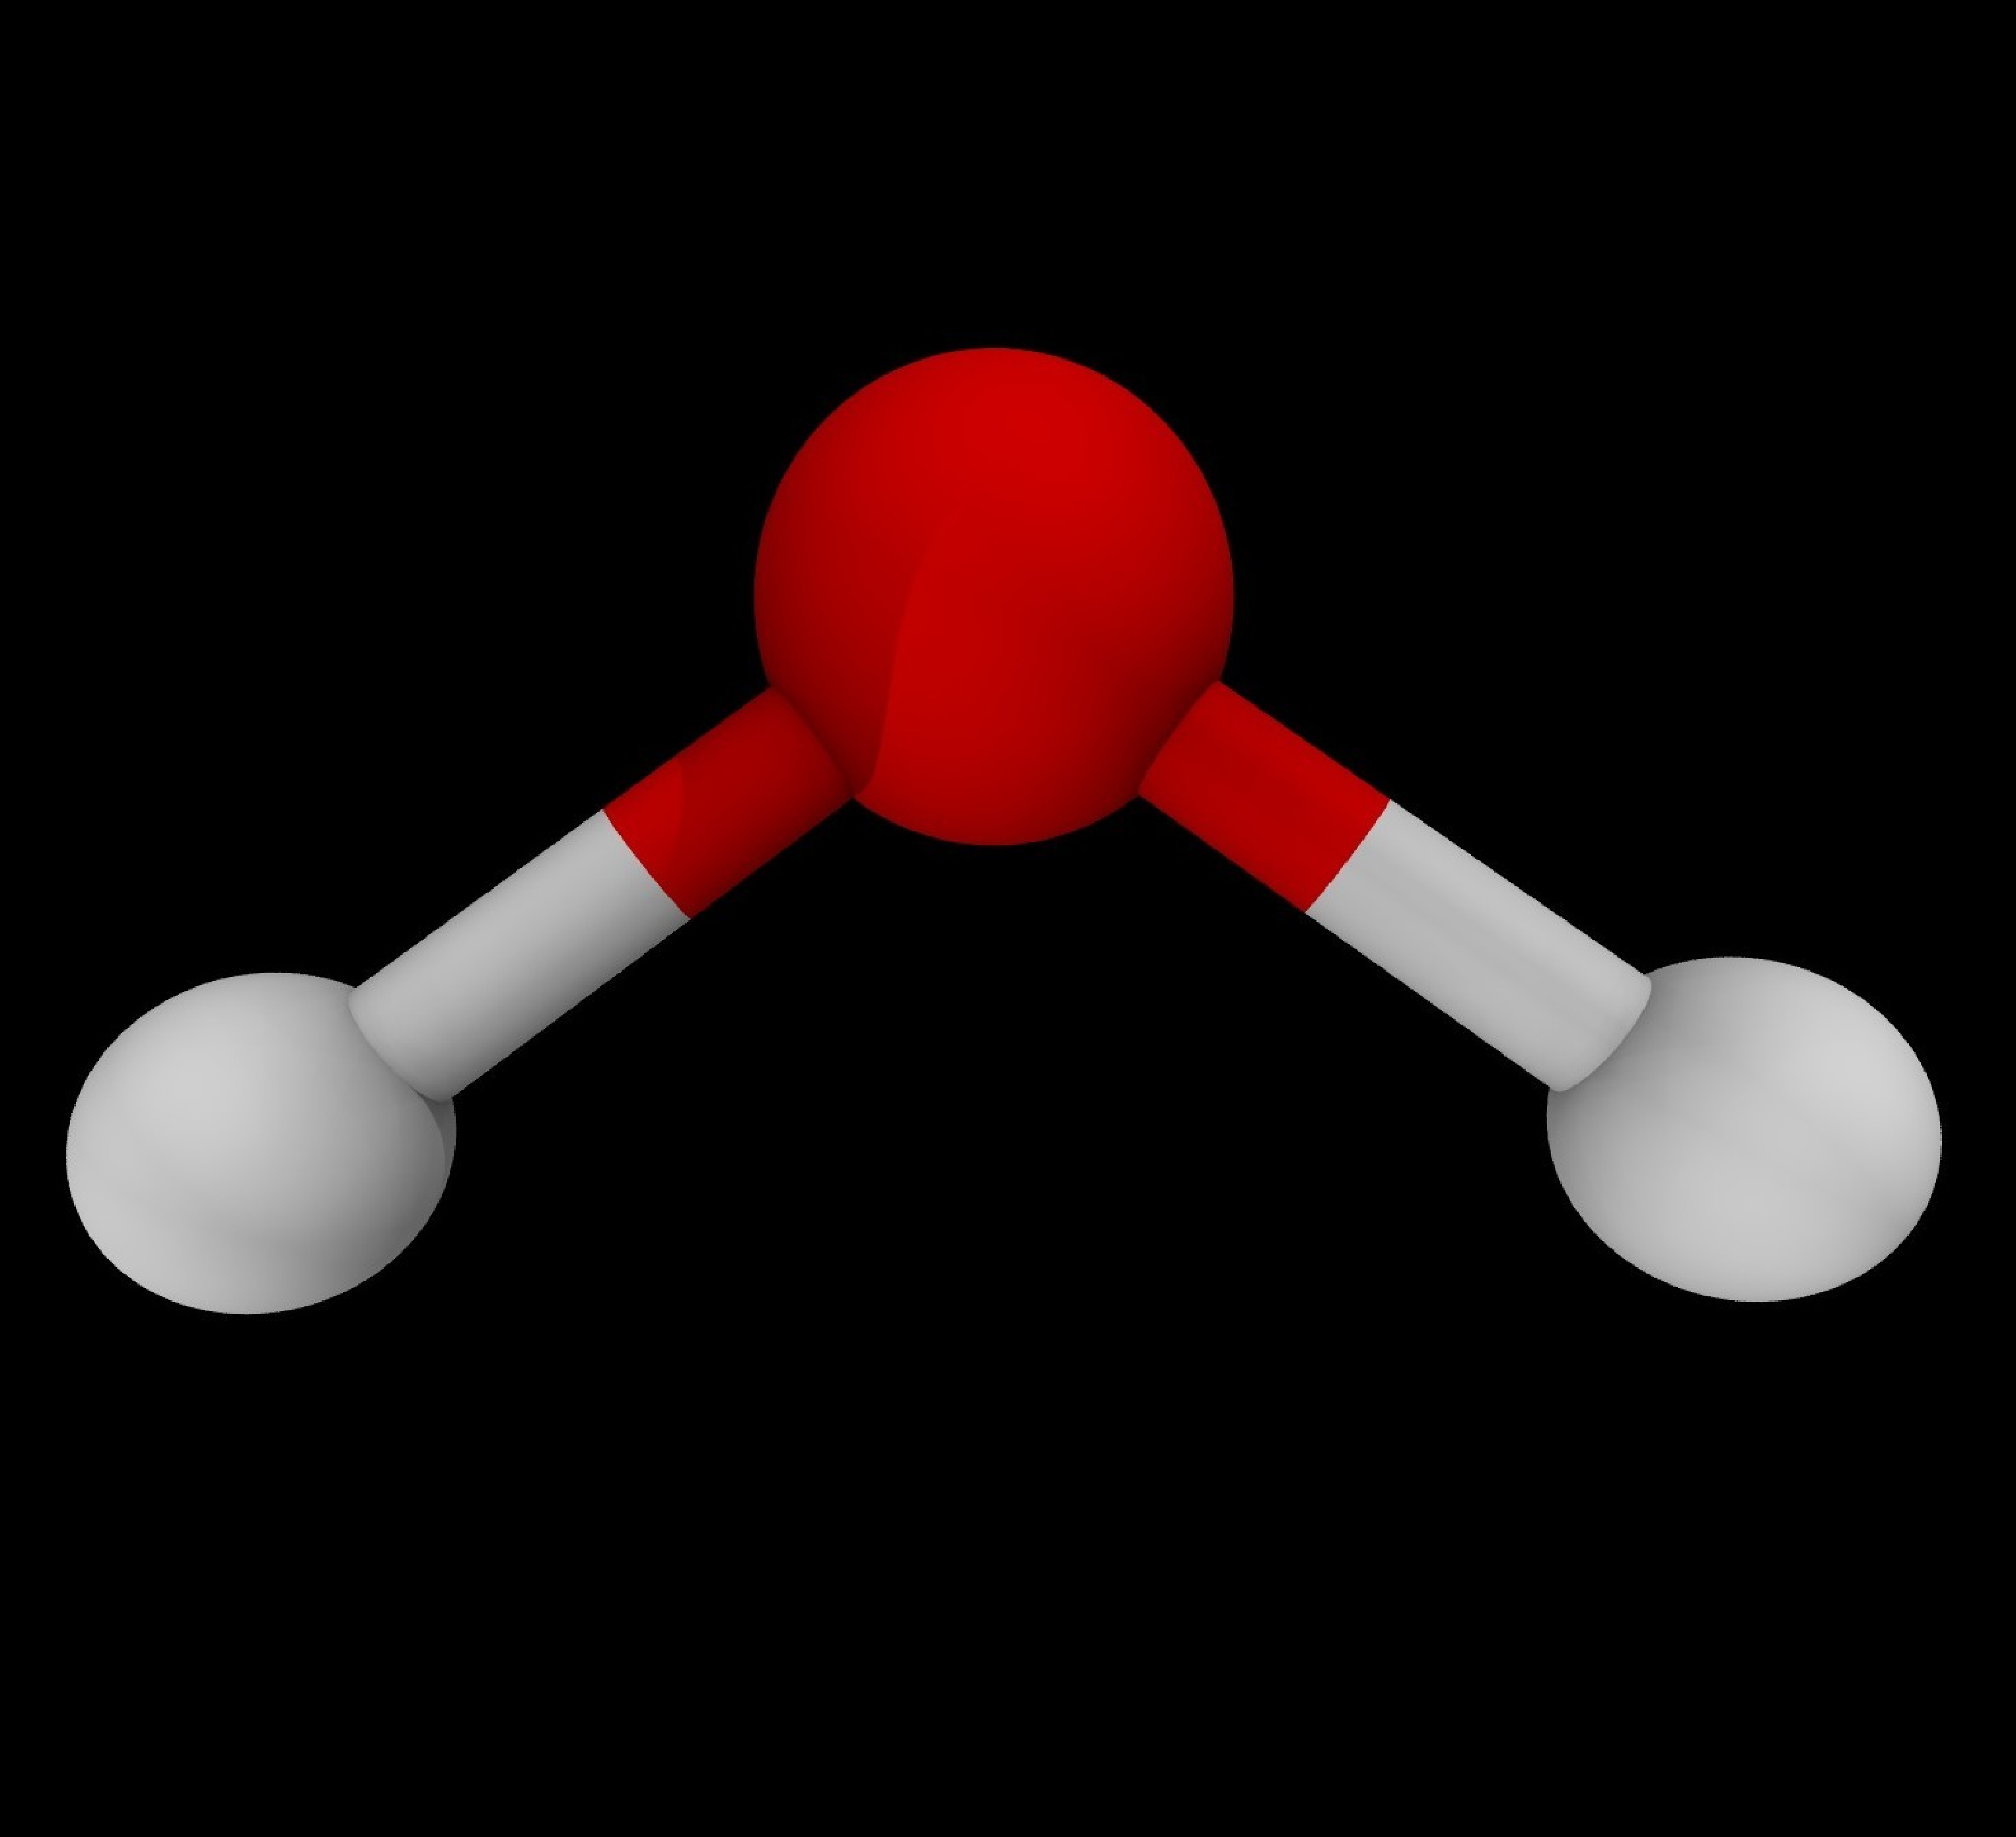
\includegraphics[width=0.52\linewidth]{../pictures/h2o_molecule.pdf}}
\subcaptionbox{Electron density representation of the water molecule. The density is caculated with the Hartree-Fock method. Taken from my simulations for a course at the University of Oslo.}{
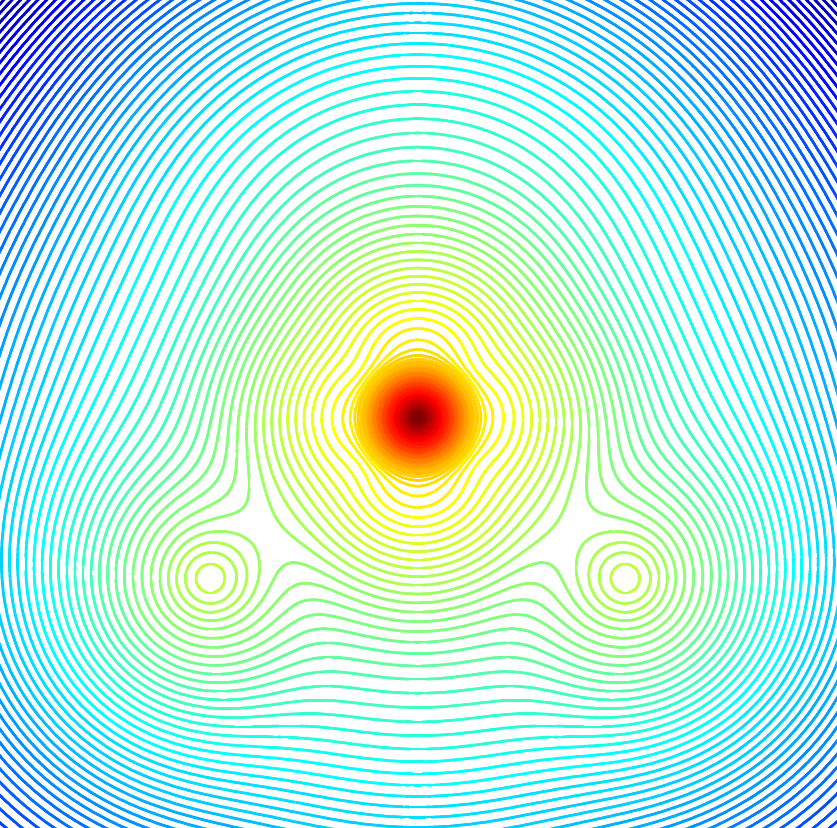
\includegraphics[width=0.48\linewidth]{../pictures/h2o_hf_density.png}}
\caption{Two perspectives on the water molecule.}
\end{minipage}
\label{fig:water_molecule}
\end{figure}

\begin{table}[h!tb]
\caption{Experimental data for the water molecule.}
\label{tb:intro:h2odata}
\begin{center}
\begin{tabular}{c|c|c}
Description & Symbol & Value \\
\hline
H-O-H angle & $\theta$ & \SI{104.52}{\degree} \\
Distance O-H & $d_{OH}$ & \SI{0.9572}{\angstrom} \\
\end{tabular}
\end{center}
\end{table}

\section{Molecular models of water}
@1933-model @TIP-models.  \citet{Vega2011} review rigid non-polarizable models.


\section{Molecular Modeling of Methane Hydrates}

\section{Molecular Modeling of Fracture}
\citet{doi:10.1142/9789812773326_0001} review some aspects of molecular modeling of fracture. 



\section{Research questions}
I will name a few outstanding quiestions. @FindFromMechPropPaper.


\begin{enumerate}
\item What is the fracture toughness of methane hydrate? Fracture toughness of matarials are usually estimated with standardized mechanical tests. Since such tests are hard to do for methane hydrates, it is actually possible that the best estimates can come from molecular simulations. 
\item What characterizes failure in methane hydrates, is it ductile or brittle? Are there sub-critical fractures, and are they available on the timescale of molecular dynamics?
\item What does the fracture surface look like?
\item Are the fracture properties of methane hydrates predictable? It could for instance be that for a given stress or strain applied to a slab of methane hydrate, the critial stress/strain or the time it takes before it starts cracking is very predictable, and sharply peaked around some value. On the other hand, it could be that statisical processes in the material are important, and that there is a wide waiting-time distribution governing the fracture initiation or even propagation.
\item Strain hardening to 20\% strain. How can this be explained?
\end{enumerate}

@TellWhatQuestionsIEndUpAnswering